\section{启动/停止服务器}\label{ux542fux52a8ux505cux6b62ux670dux52a1ux5668}

StarRiver
安装完成后会在后台自动运行。如您需要人工控制服务器启停,可以使用开始菜单中建立快捷方式来操作。

\begin{figure}[htbp]
\centering
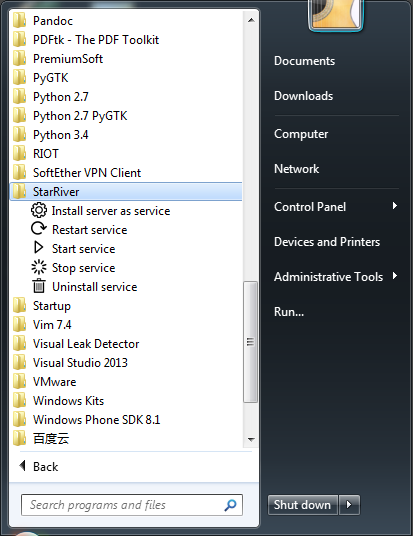
\includegraphics{../img/shortcuts.png}
\end{figure}

五个快捷方式功能分别如下:

\begin{itemize}
\itemsep1pt\parskip0pt\parsep0pt
\item
  \textbf{Install server as service}:将 StarRiver 服务器安装为 Windows
  服务,可以在后台运行。安装程序默认已经执行了此操作。
\item
  \textbf{Restart service}:手动重启 StarRiver 服务。
\item
  \textbf{Start service}:手动启动 StarRiver 服务。
\item
  \textbf{Stop service}:手动停止 StarRiver 服务。
\item
  \textbf{Uninstall service}:删除 StarRiver Windows 服务。StarRiver
  服务器本身不会被删除,但无法再随 Windows 自动启动。
\end{itemize}
